\section{The Problem as a Graph}\label{sec:asgraph-\myInitials}

% Discuss here how instances of that problem can be expressed as a graph.

We can formalize the above problem as a complex, heterogeneous network with the following structure:

\begin{center}
    \parbox[t]{2.4in}{
        \raggedright%
        \textbf{\textit{Node Types :}}
        \begin{enumerate}[topsep=0pt,itemsep=-2pt,leftmargin=13pt]
            \item Airport
            \item Seaport
            \item Rail Station
        \end{enumerate}
    }%
    \parbox[t]{2.4in}{
        \raggedright%
        \textbf{\textit{Edge Properties :}}
        \begin{enumerate}[topsep=0pt,itemsep=-2pt,leftmargin=13pt]
            \item Direction
            \item Transition Probability ($p_1...p_k$)
            \item Distance
            \item Travel Time
        \end{enumerate}
    }
\end{center}

\begin{figure}[h]
\centering
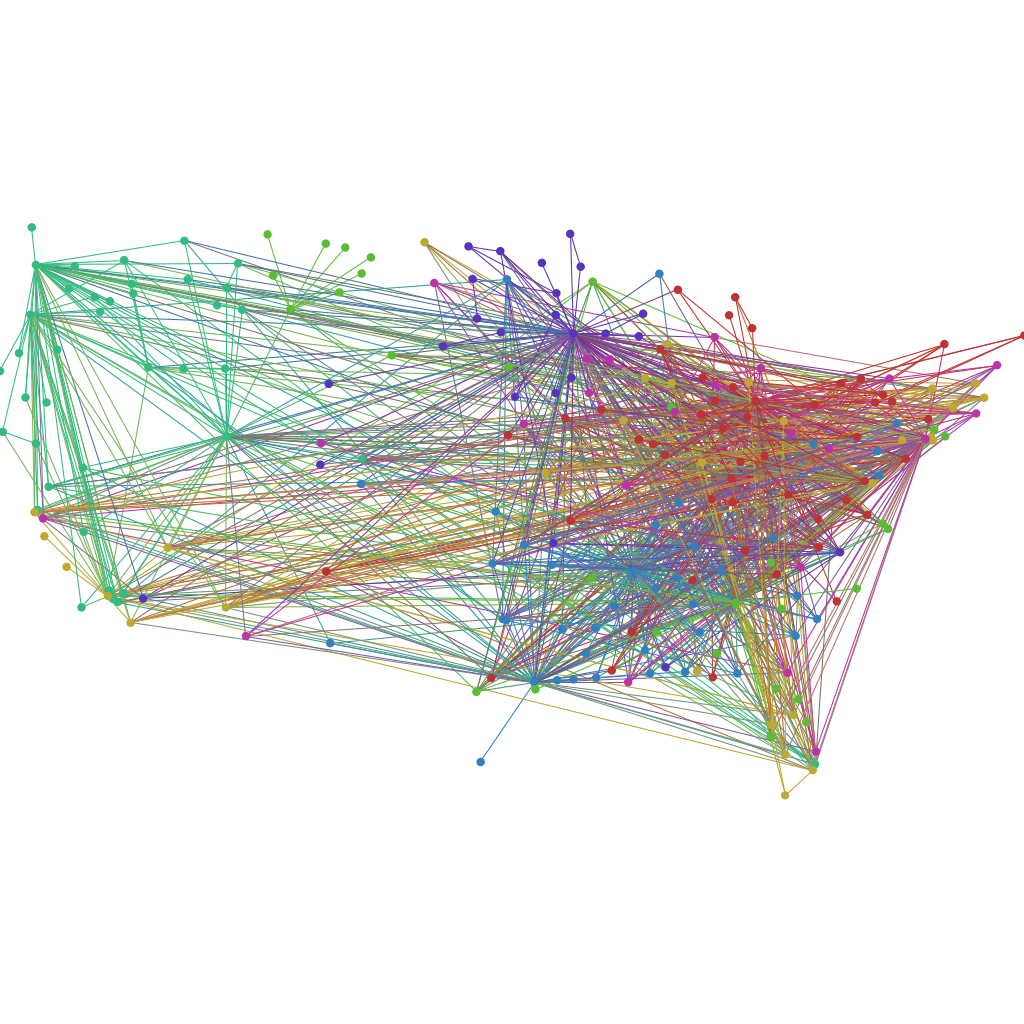
\includegraphics[width=0.7\textwidth]{figures-RW/usairport_base.png}
    \caption{ \centering
        The US Domestic Flight Network\cite{stanford_dhs} - Shows the US subset of the SNAP US and Canada Airport data set\cite{snapnets} in Table \ref{table:potential_datasets}. Nodes are airports, edges are the connections between them. Edge are colored relative to the frequency of travel between incident airports.
    }
    \label{fig:us_domestic}
\end{figure}

\newpage


